\documentclass[handout,aspectratio=169]{beamer}
\usepackage{graphicx}
\usepackage{booktabs}
\usepackage{array}
\usepackage{listings}
\usepackage{xcolor}

\definecolor{codegreen}{rgb}{0,0.6,0}
\definecolor{codegray}{rgb}{0.5,0.5,0.5}
\definecolor{codepurple}{rgb}{0.58,0,0.82}
\definecolor{backcolour}{rgb}{0.95,0.95,0.92}

\lstset{
    backgroundcolor=\color{backcolour},
    commentstyle=\color{codegreen},
    keywordstyle=\color{magenta},
    numberstyle=\tiny\color{codegray},
    stringstyle=\color{codepurple},
    basicstyle=\ttfamily\scriptsize,
    breakatwhitespace=false,
    breaklines=true,
    captionpos=b,
    keepspaces=true,
    numbers=left,
    numbersep=5pt,
    showspaces=false,
    showstringspaces=false,
    showtabs=false,
    tabsize=2
}

\title{Perturb-Seq Reanalysis Pipeline}
\date{2026-06-04}
\author{Kirill Tsukanov \\ Senior Full Stack Developer \& Data Engineer \\ \texttt{ktsukanov@ebi.ac.uk}}

\setbeamertemplate{navigation symbols}{}
\setbeamertemplate{footline}{%
  \begin{beamercolorbox}[wd=\paperwidth,ht=2.5ex,dp=1.5ex,center]{}
    \hspace{15pt}\usebeamerfont{author in head/foot}Perturb-Seq Reanalysis Pipeline
    \hfill
    \usebeamerfont{date in head/foot}\insertframenumber{} / \inserttotalframenumber
    \hspace{15pt}
  \end{beamercolorbox}%
}

\begin{document}

\begin{frame}
    \titlepage
\end{frame}

\begin{frame}{What is Perturb-Seq?}
    \centering
    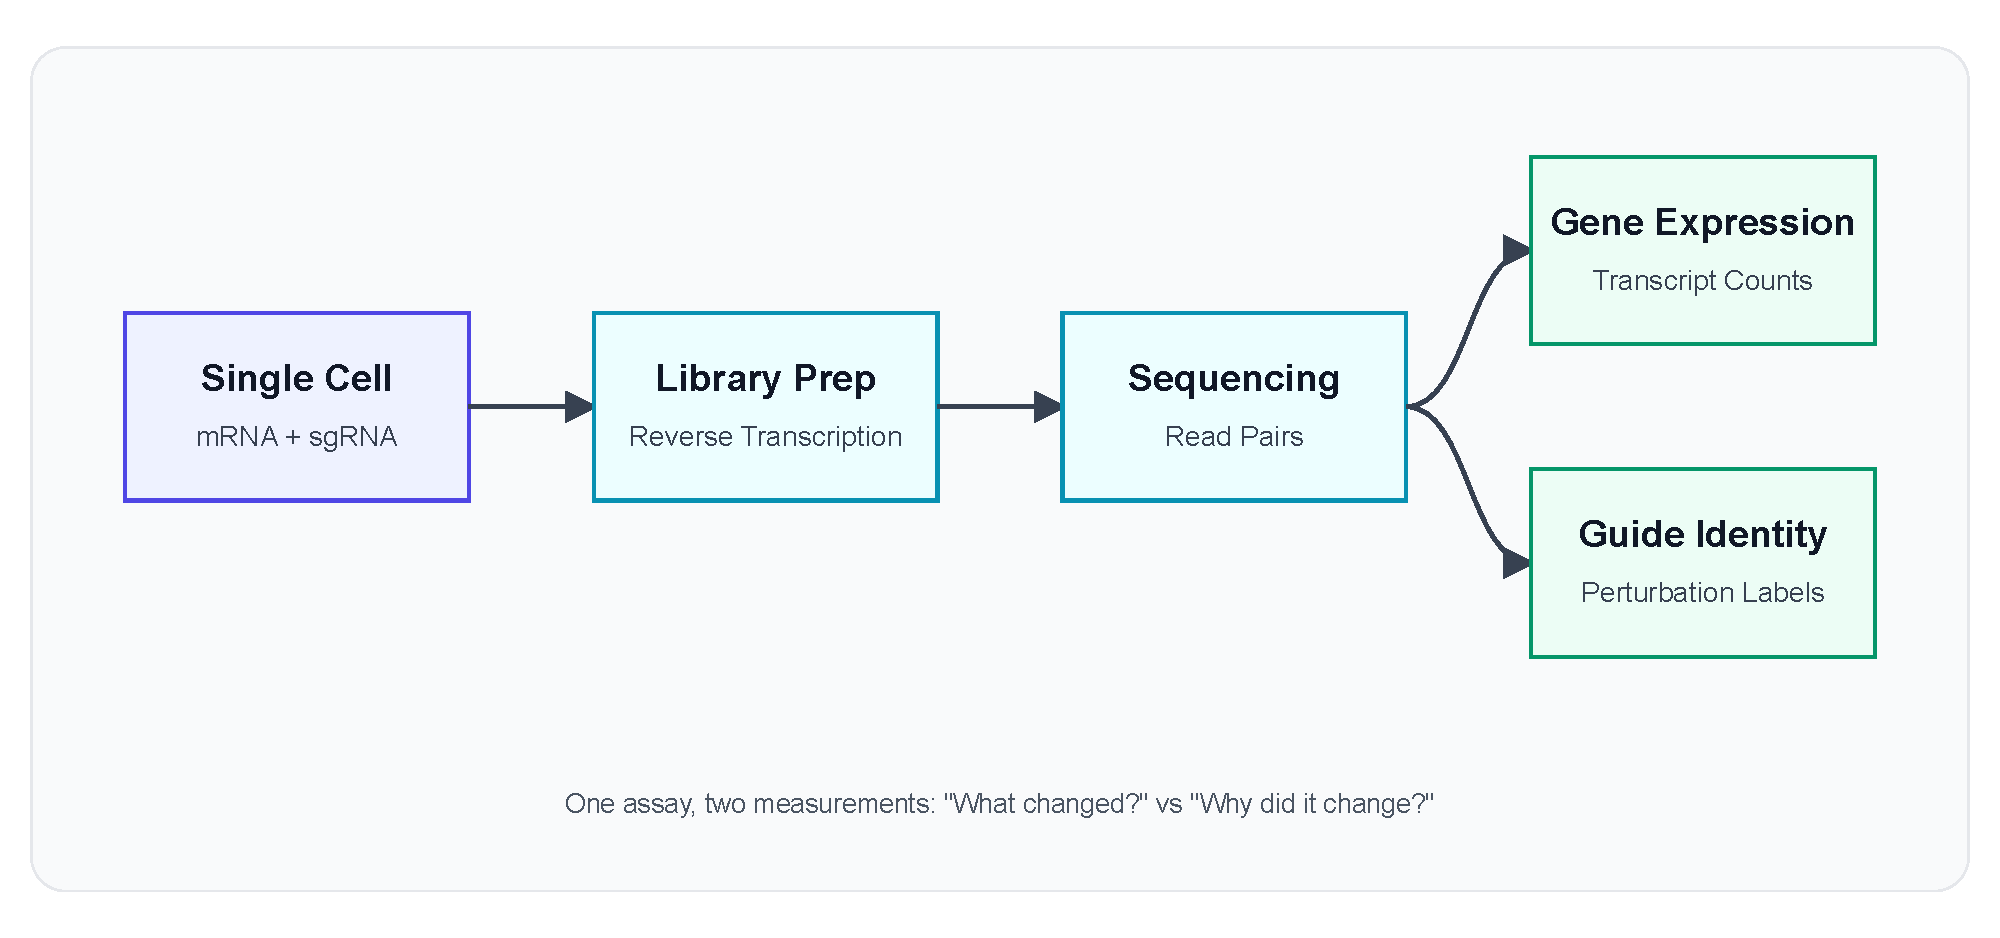
\includegraphics[width=0.98\linewidth,height=0.78\textheight,keepaspectratio]{what_is_perturb_seq.pdf}
\end{frame}

\begin{frame}{Why re-process from FASTQ?}
    \begin{itemize}
        \item \textbf{Main problem:} scPerturb datasets are usually made available as processed H5AD files, but they come from different pipelines, references, and filtering choices.
        \item \textbf{Stable schema:} Re-processing gives us a common count matrix layout, common metadata expectations, and a consistent way to attach guide counts. This significantly simplifies downstream analysis.
        \item \textbf{Quality control:} Raw reads let us apply the same checks across studies instead of inheriting every author-specific decision.
        \item \textbf{Batch effects:} Reprocessing from scratch using a unified pipeline helps in reducing systematic batch effects between datasets.
        \item \textbf{Catalogue expectation:} Users expect harmonised data in the Perturbation Catalogue, not only links to heterogeneous processed files.
    \end{itemize}
\end{frame}

\begin{frame}{Why Kallisto + Bustools?}
    \begin{itemize}
        \item \textbf{Speed:} Kallisto + Bustools is much faster than Cell Ranger while giving very comparable expression quantification.
        \item \textbf{Resource fit:} We have adequate, but not unlimited, compute and storage. The pipeline must work within those limits.
        \item \textbf{Full catalogue scale:} We want to process all datasets we have, and be able to reprocess them if the pipeline improves.
        \item \textbf{Future-proofing:} New Perturb-Seq datasets are expected to be very large, so the pipeline needs to scale well rather than depend on throwing more hardware at each run.
    \end{itemize}
\end{frame}

\begin{frame}{Pipeline Architecture}
    \centering
    
\includegraphics[width=0.98\linewidth,height=0.78\textheight,keepaspectratio]{pipeline_workflow.pdf}
\end{frame}

\begin{frame}{Downstream analysis}
    \centering
    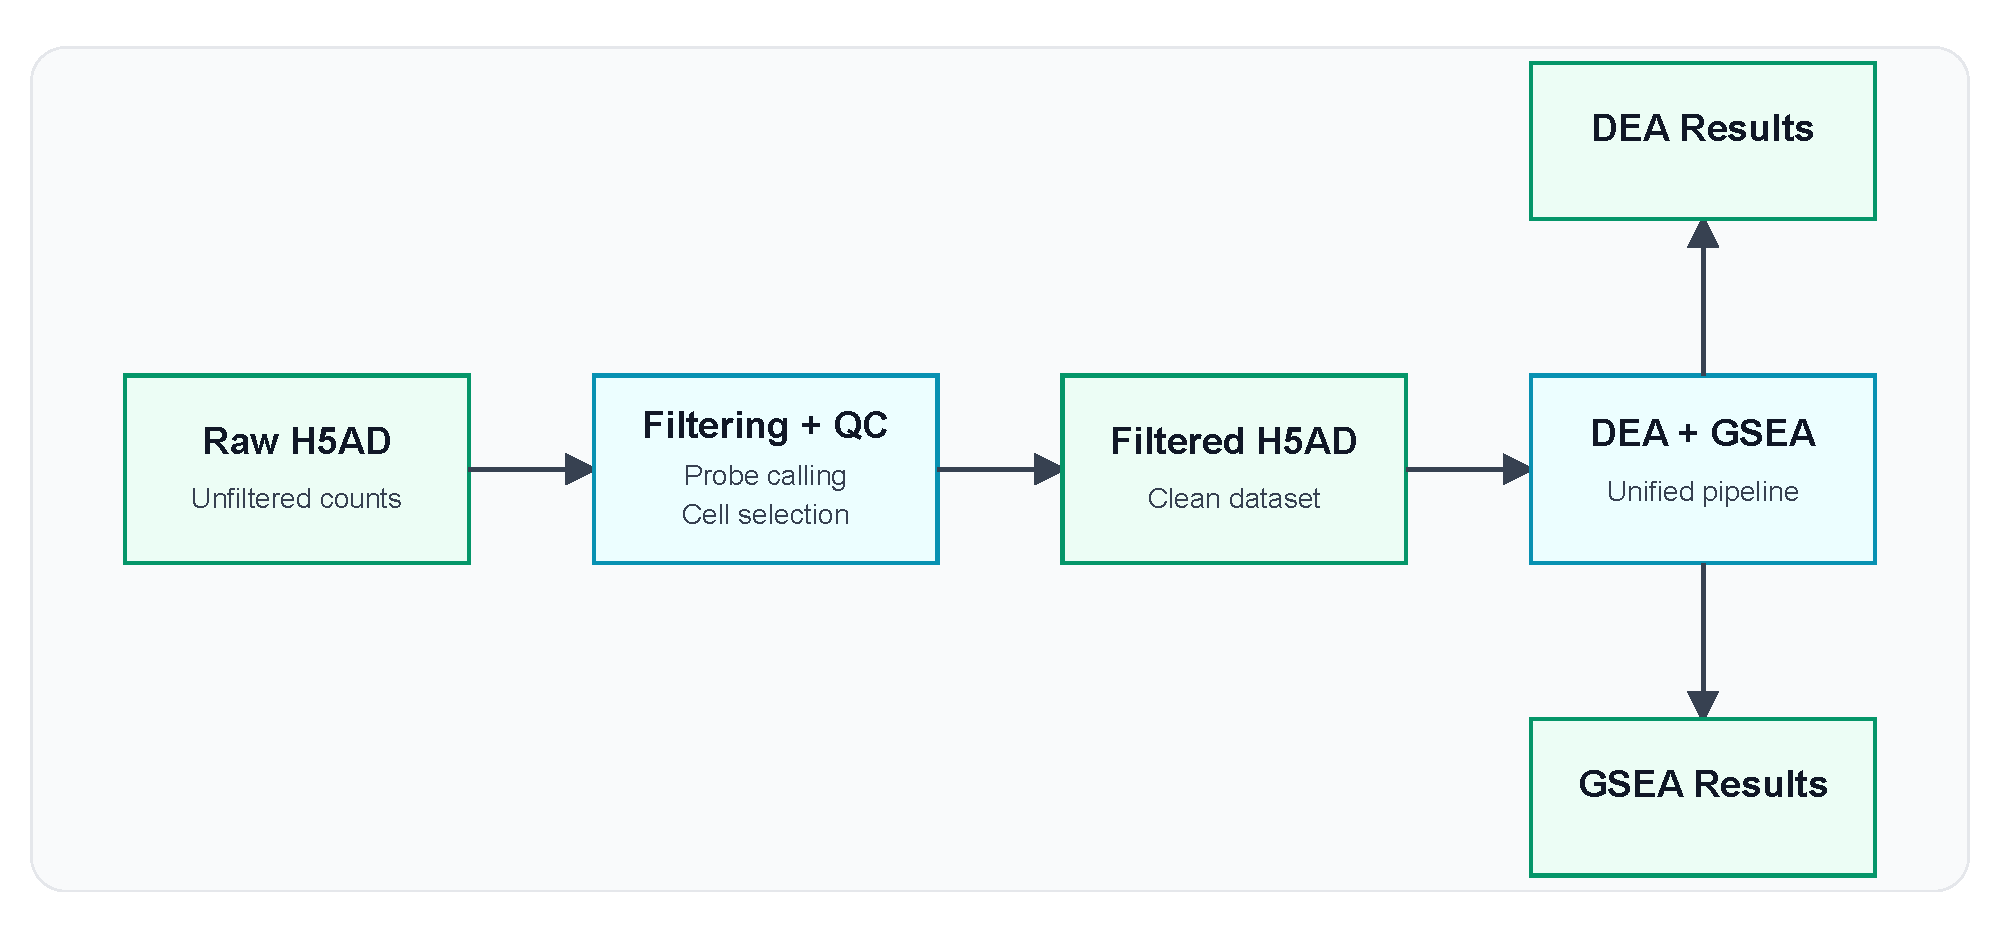
\includegraphics[width=0.98\linewidth,height=0.78\textheight,keepaspectratio]{downstream_analysis.pdf}
\end{frame}

\begin{frame}{Challenges}
    \begin{itemize}
        \item \textbf{ENA FASTQs missing technical reads:} Historical ENA FASTQs for this dataset do not include the barcode/UMI reads. Current workaround: SRA download with technical reads included. We notified ENA; they are aware and plan to fix it, so future runs may use ENA directly.
        \item \textbf{Sample grouping:} SRRs and lanes must be grouped by physical well before counting. This is currently parsed from ENA library names; later versions may autodetect this.
        \item \textbf{Barcode collisions:} Final concatenation adds sample suffixes so identical 10x barcodes from different wells remain distinct.
        \item \textbf{GEX/KITE matching:} Guide barcodes are not exactly the same as expression barcodes in this dataset. The pipeline applies the required KITE barcode correction before alignment.
    \end{itemize}
\end{frame}

\begin{frame}{List of datasets}
    \centering
    \scriptsize
    \begin{tabular}{lrrrrrr}
        \toprule
        Dataset & Size (TB) & Total cells & Single-gene & Control & Multi-gene & No-guide \\
        \midrule
        Nadig 2025 Jurkat & 2.0 & 588,498 & 214,092 & 10,629 & 289,965 & 58,565 \\
        Nadig 2025 HepG2 & 2.6 & 501,121 & 129,909 & 4,835 & 333,994 & 21,803 \\
        Replogle 2022 K562 Essential & 1.7 & 544,799 & 274,155 & 11,048 & 191,241 & 61,211 \\
        Replogle 2022 K562 GW & 11.0 & 1,314,345 & 613,755 & 29,463 & 545,514 & 101,360 \\
        Replogle 2022 RPE1 Essential & 1.9 & 509,962 & 206,740 & 11,855 & 197,064 & 79,695 \\
        \bottomrule
    \end{tabular}
    \vspace{1em}
    \begin{itemize}
        \item Currently, 5 datasets are processed.
        \item Gaussian-Poisson threshold used for guide calling (8-9 UMI).
    \end{itemize}
\end{frame}

\begin{frame}{Cell-Level Expression Agreement}
    \begin{columns}[T,onlytextwidth]
        \begin{column}{0.49\textwidth}
            \centering
            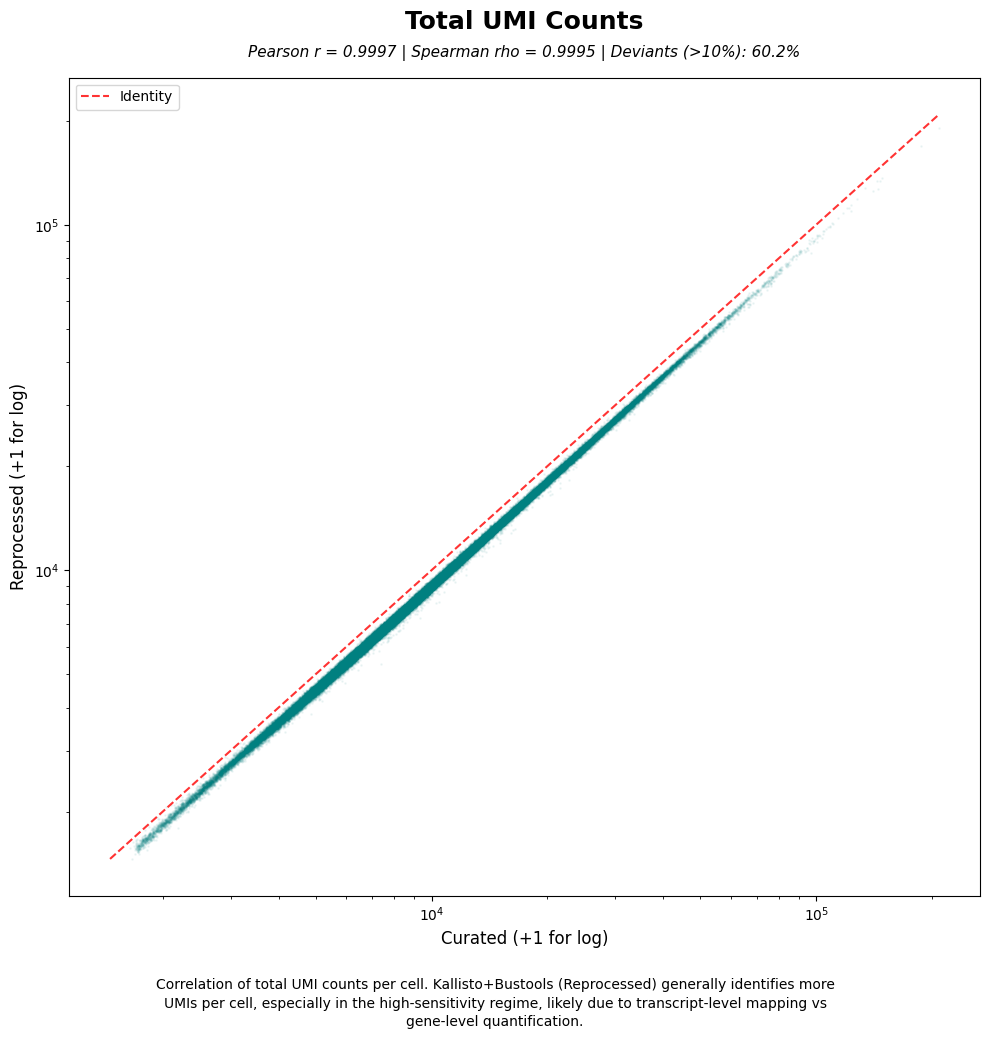
\includegraphics[width=\linewidth,height=0.78\textheight,keepaspectratio]{umi.png}
        \end{column}
        \begin{column}{0.49\textwidth}
            \centering
            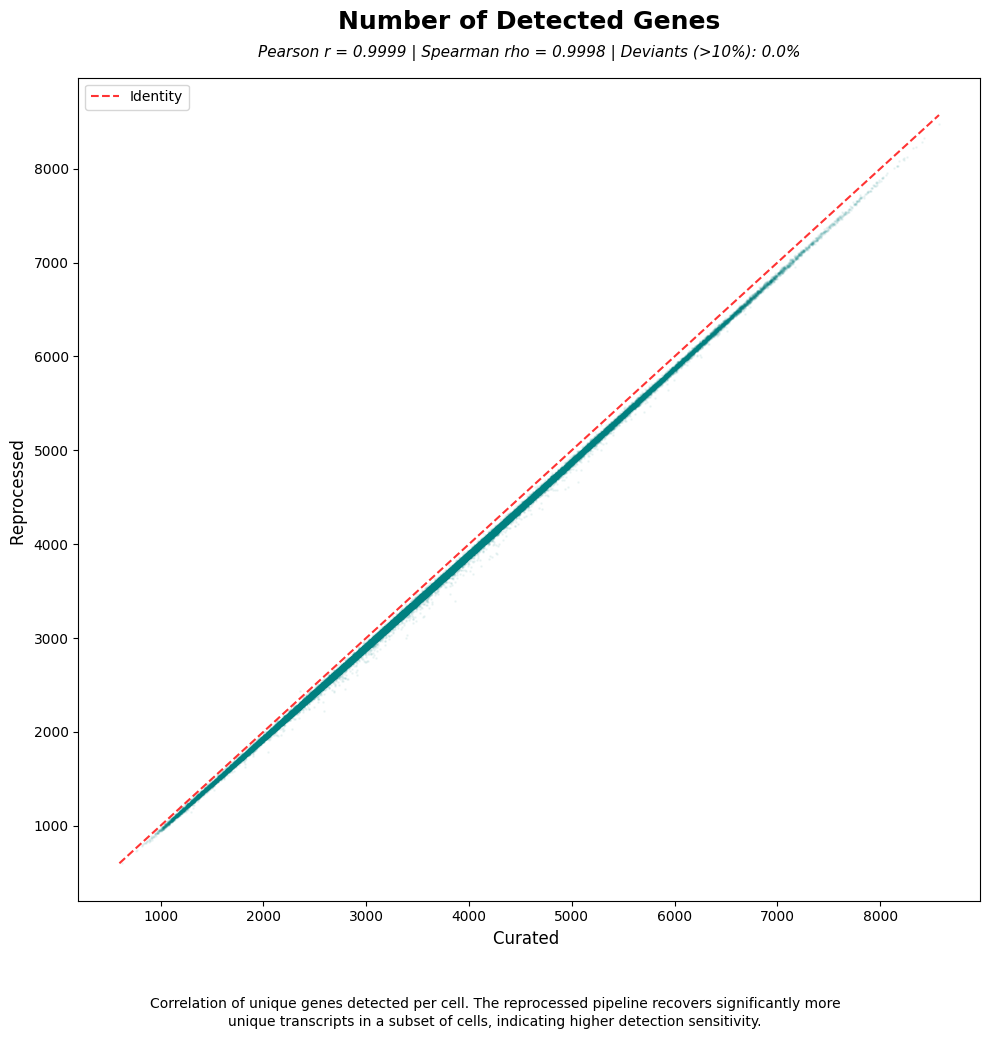
\includegraphics[width=\linewidth,height=0.78\textheight,keepaspectratio]{genes.png}
        \end{column}
    \end{columns}
\end{frame}

\begin{frame}{Gene-Level Expression Agreement}
    \begin{columns}[T,onlytextwidth]
        \begin{column}{0.49\textwidth}
            \centering
            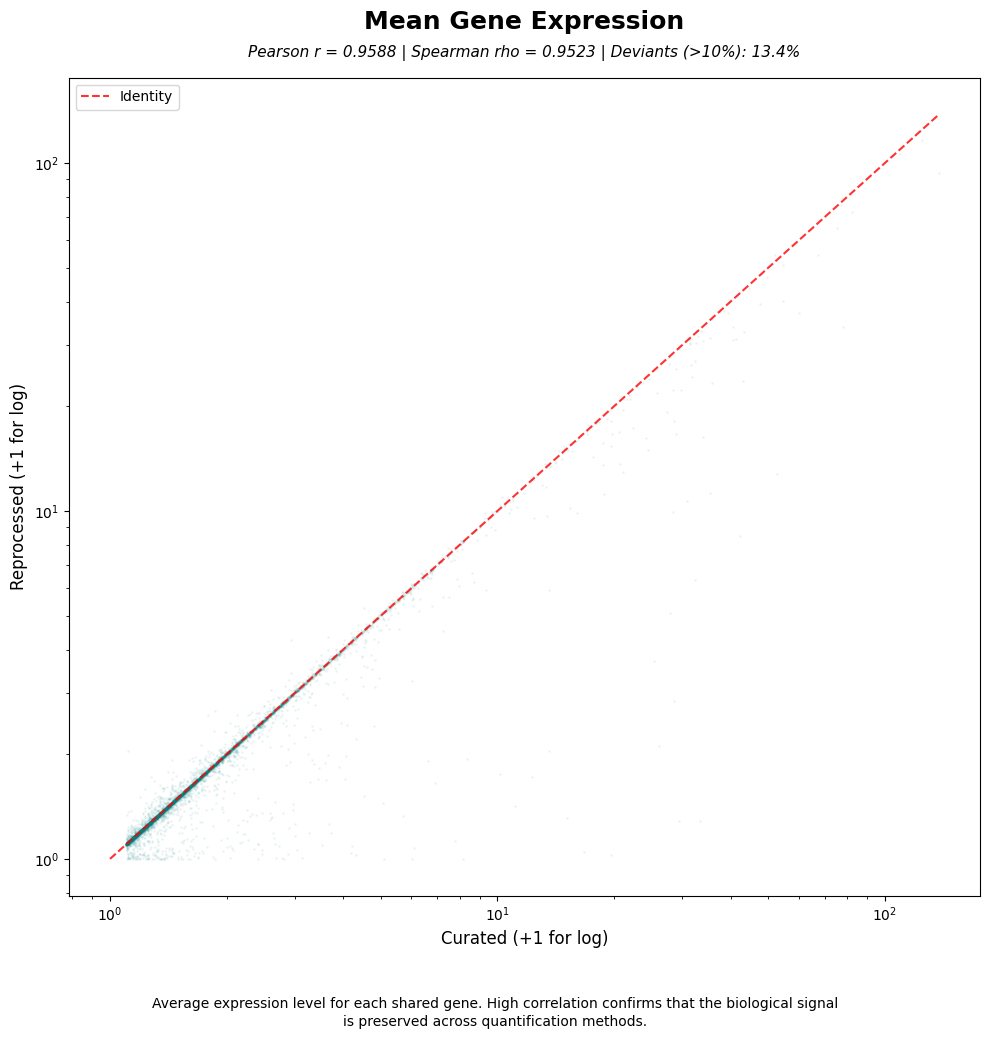
\includegraphics[width=\linewidth,height=0.78\textheight,keepaspectratio]{expression.png}
        \end{column}
        \begin{column}{0.49\textwidth}
            \centering
            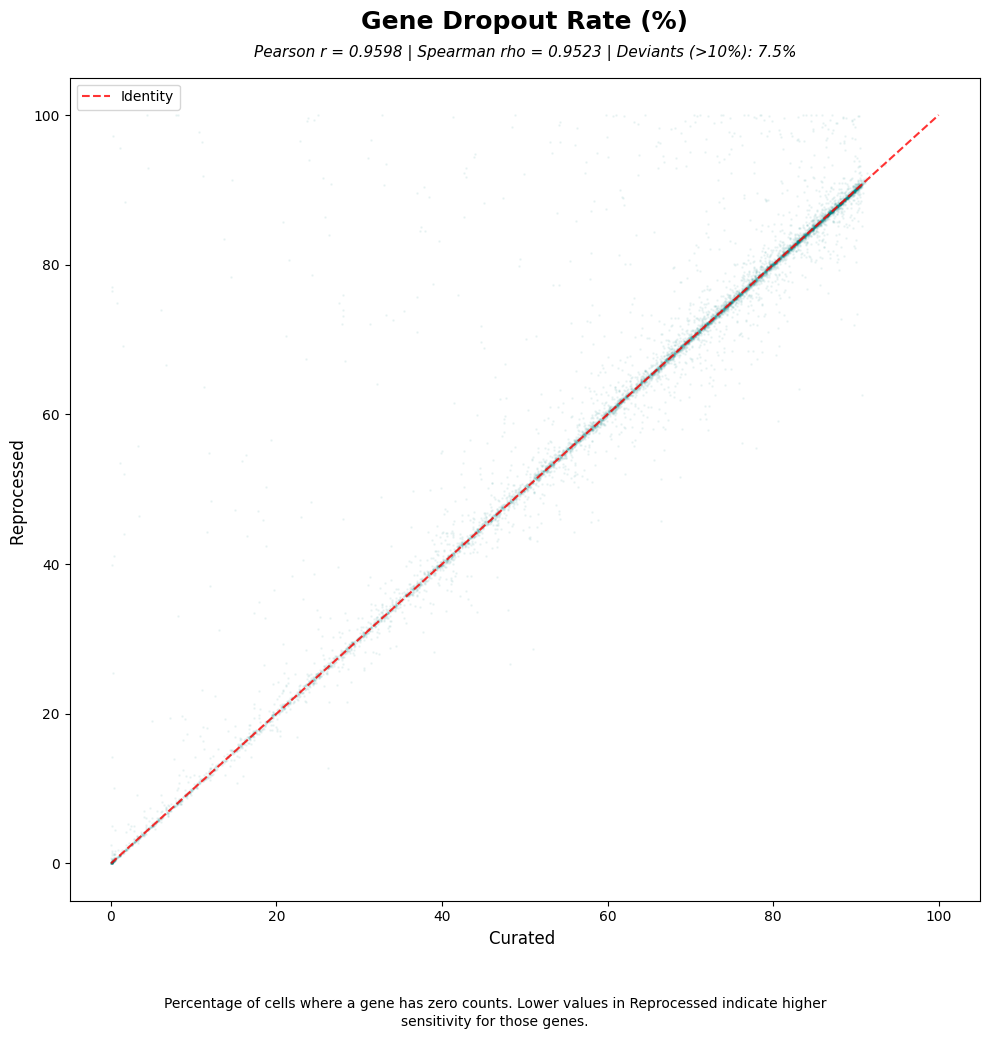
\includegraphics[width=\linewidth,height=0.78\textheight,keepaspectratio]{dropout.png}
        \end{column}
    \end{columns}
\end{frame}

\begin{frame}{Expression Vectors Are Preserved}
    \begin{itemize}
        \item For each shared cell, we compare the original and reprocessed expression vectors over the same genes.
        \item The histogram shows the distribution of Pearson correlation values for a sample of 10,000 cells.
    \end{itemize}
    \vspace{0.5em}
    \centering
    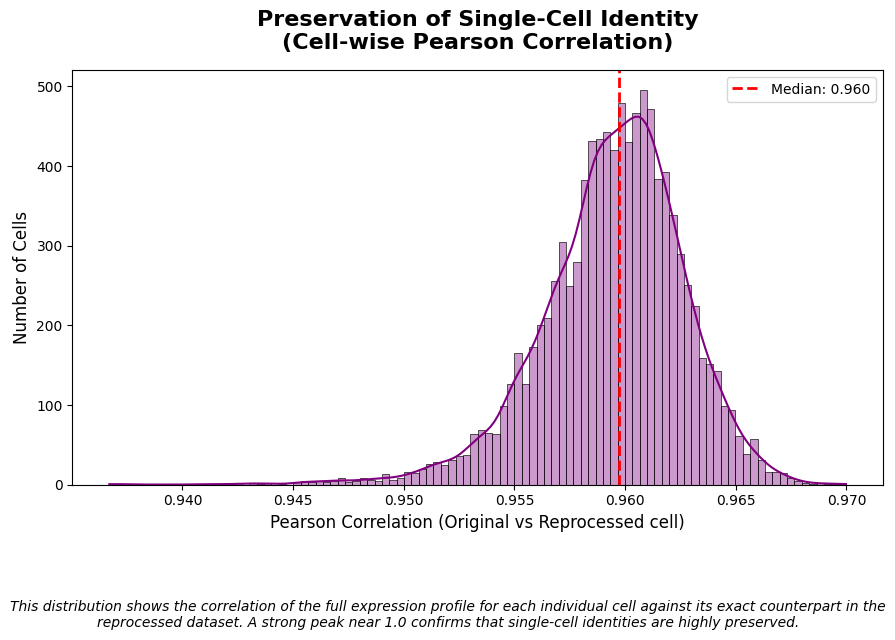
\includegraphics[width=0.7\linewidth,height=0.6\textheight,keepaspectratio]{pearson_per_cell.png}
\end{frame}

\begin{frame}{Guide Recovery: Mixture Model Approach}
    \begin{itemize}
        \item We use a \textbf{Gaussian-Poisson mixture model} to separate guide signal from background.
        \item The background is modeled as a Poisson distribution, while the true signal follows a Gaussian distribution.
        \item The decision threshold is automatically set at the crossover point where the probability of signal becomes higher than background.
        \item Cells are assigned a guide if at least one probe targets the gene and passes this threshold.
        \item $>$95\% overall agreement on call outcomes between original and reprocessed data; for single gene cells, $>$99.8\% agreement.
    \end{itemize}
\end{frame}

\begin{frame}{What We Have Now}
    \begin{itemize}
        \item A working, reproducible FASTQ-to-H5AD pipeline for Perturb-Seq datasets.
        \item Both expression and guide calling are solved with very good alignment to original data.
        \item A comparison workflow that checks cell-level expression, gene-level expression, dropout, and perturbation labels.
        \item DEA and GSEA downstream analysis.
        \item Full pipeline was successfully ran for 5 datasets in the Catalogue.
    \end{itemize}
\end{frame}

\begin{frame}{Next Steps}
    \begin{itemize}
        \item Further exploration and validation of results.
        \item Updating data in Catalogue and publishing a new release.
        \item Expand pipeline to deal with more datasets, 10x v2 chemistry, CSP data.
        \item Eventually: release pipeline as a separate package.
    \end{itemize}
\end{frame}

\end{document}
